
\section{Implementation}

Figure~\ref{fig:prototype_component_overview} shows an abstract overview of communication between the chatbot and Facebook Messenger servers. The user interacts with the chatbot using the Facebook Messenger platform on either a mobile phone or website. When the user sends a message to the chatbot it is sent to Facebook servers that decide what chatbot application to forward the message onto. The message comes in a \textit{json} format that is parsed by the chatbot application to understand how the user interacted and what message was sent. The chatbot reads and writes the necessary information into the PostgreSQL database to decide a response. When it is ready, it sends a request to the Facebook servers that forward it onto the user's Facebook Messenger account that can be read from the Messenger platform. All code is open-source and hosted on \textit{GitHub} (\url{www.github.com/harrymt/harryshabits}).

\begin{figure}[H]
    \centering
    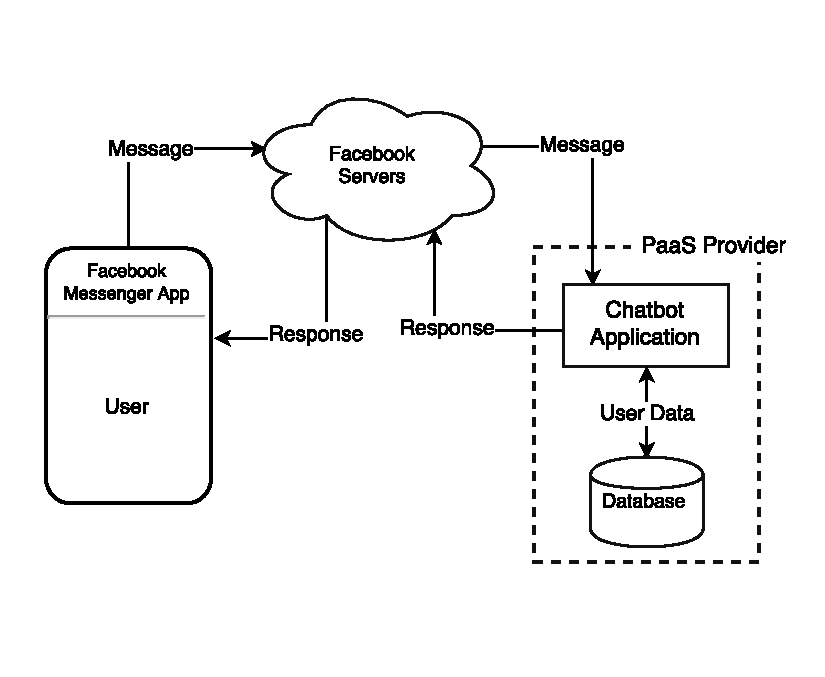
\includegraphics[width=5.1in]{../resources/diagrams/chatbot-component-overview.pdf}
    \caption{Prototype Component Overview}
    \label{fig:prototype_component_overview}
\end{figure}

The prototype was developed in \textit{node.js} (\url{www.nodejs.org}), built on the Facebook Messenger chatbot platform and hosted on \textit{Heroku} (\url{www.heroku.com}) a free PaaS (Platform-as-a-Service) option. Facebook messenger encourages developers to create bots to interact with their users as these bots act as a real person with similar interaction flow, plus a few additional features, such as \textit{Quick Replies}~\cite{doc_fb_quick_replies} for revealing a list of options to a user. Simple call and responses were used to interact with users and track their data instead of NLP to limit the scope of the project. The bot also tracked various data about how people logged their habits, such as what day they tracked their habit and how many times they delayed their checking messages. Heroku provides 10,000 rows as their free option in a \textit{PostgreSQL} (\url{https://www.postgresql.org/}) database. Figure~\ref{fig:db_diagram} outlines each database table with what information is stored. The \textit{Facebook ID} is used to identify each user and what habits they tracked. When a user has told the bot they completed their habit, a new row in the \textit{Habits} table would be added and linked to the user in the \textit{Users} table. Two global variables are used to maintain the state across local and live versions of the system to display the length of study and if it is active.

\begin{figure}[H]
    \centering
    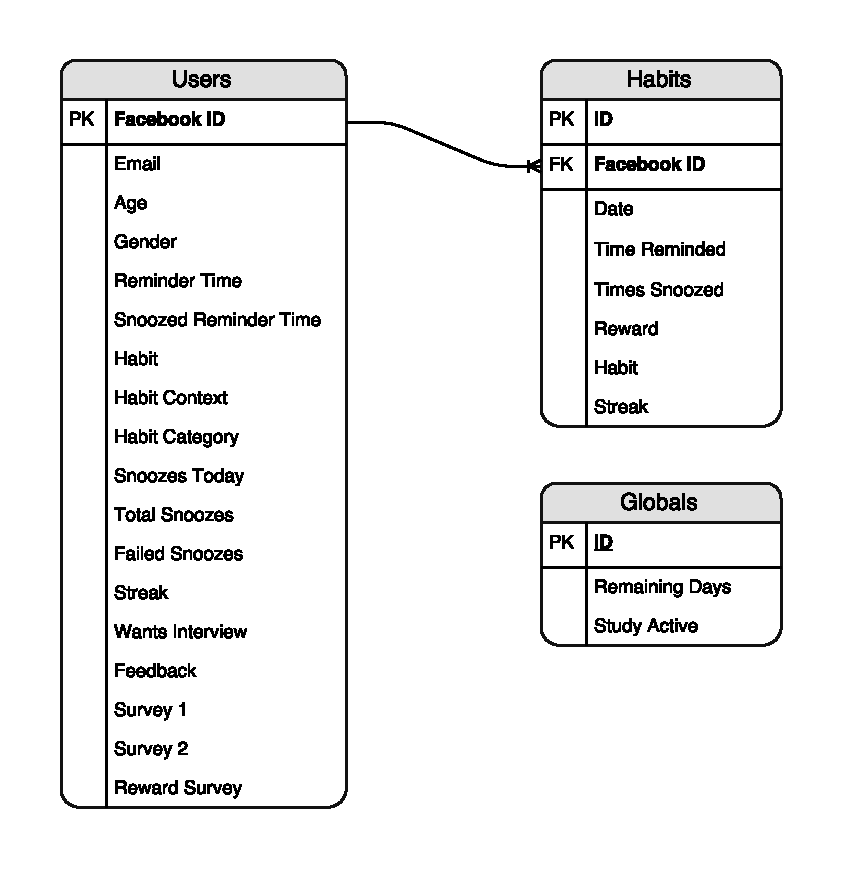
\includegraphics[width=5in]{../resources/diagrams/database-diagram.pdf}
    \caption{Database Table Entity Relationship}
    \label{fig:db_diagram}
\end{figure}

Different languages, server, hosting provider and database provider were considered. JavaScript with node.js on Heroku with PostgreSQL were chosen because of the following reasons: node.js enables us to share the same language for the server and the client; large amount of packages to handle client and server side functionality; suitable for prototyping and rapid product iteration; Heroku has a free-tier which allows full deployment with a PostgreSQL database of up to 10,000 rows; Heroku hosts the application in the cloud, giving benefits for scalable deployments that benefit any potential future application growth. Finally, \textit{Airtable} (\url{www.airtable.com})---a database integration was integrated, however, it only provided 3,000 free rows and therefore was discarded in favour of Herokus PostgreSQL database.

\subsection*{Chatbot Overview}
When Facebook servers forward a message from the user, it could come in two forms. A simple string of characters with a Facebook ID (\textit{fbid}) or a Quick Reply key with a Facebook ID.

TODO THIS NEXT SECTION

\verb|read()|---


\verb|getUser()|---


\verb|send()|---


\verb|updateUser()|---


A scheduler was used to send backup notifications to each user after their existing routine. Heroku uses a scheduler (\url{}) to handle this process.


However, the chatbot did not account for limitations with timezone...\newline


\begin{figure}[H]
    \centering
    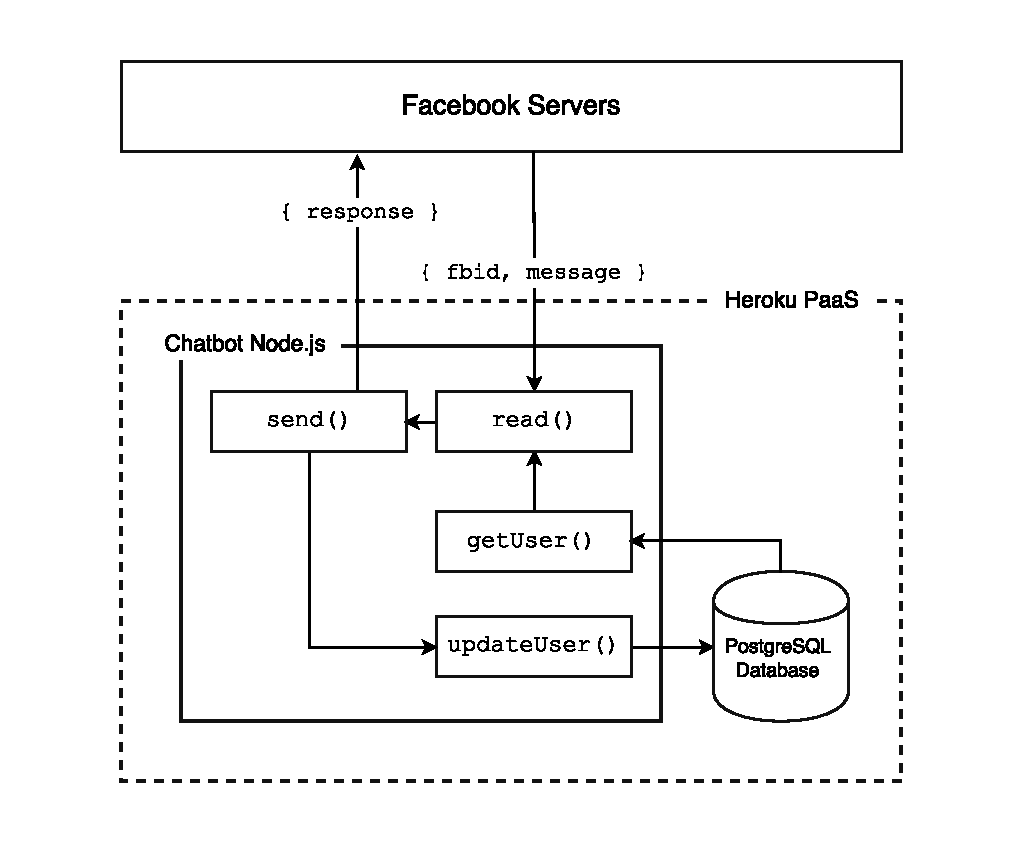
\includegraphics[width=6in]{../resources/diagrams/chatbot-detailed-overview.pdf}
    \caption{Detailed Overview}
    \label{fig:prototype_detailed_overview}
\end{figure}


\subsection*{Technical Issues}
Throughout the implementation process different techniques were explored to implement the design.
Some of the research areas were not used in the final prototype due to technical issues and limitations with the approach.


Sometimes Facebook servers would send the same message to the chatbot application twice. This would mean the reply would also be sent twice back to users. This issue was very rare and only occurred in a handful of cases and therefore was consider minor. However, it did effect this similar issue when handling free text from users. When the bot asked users to enter in a free text, e.g. email, a flag would be set to wait for free text input of that type. However, if duplicate messages were sent at this time, the application would assume users did not enter anything for the free text and would continue.

\begin{figure}[H]
    \centering
    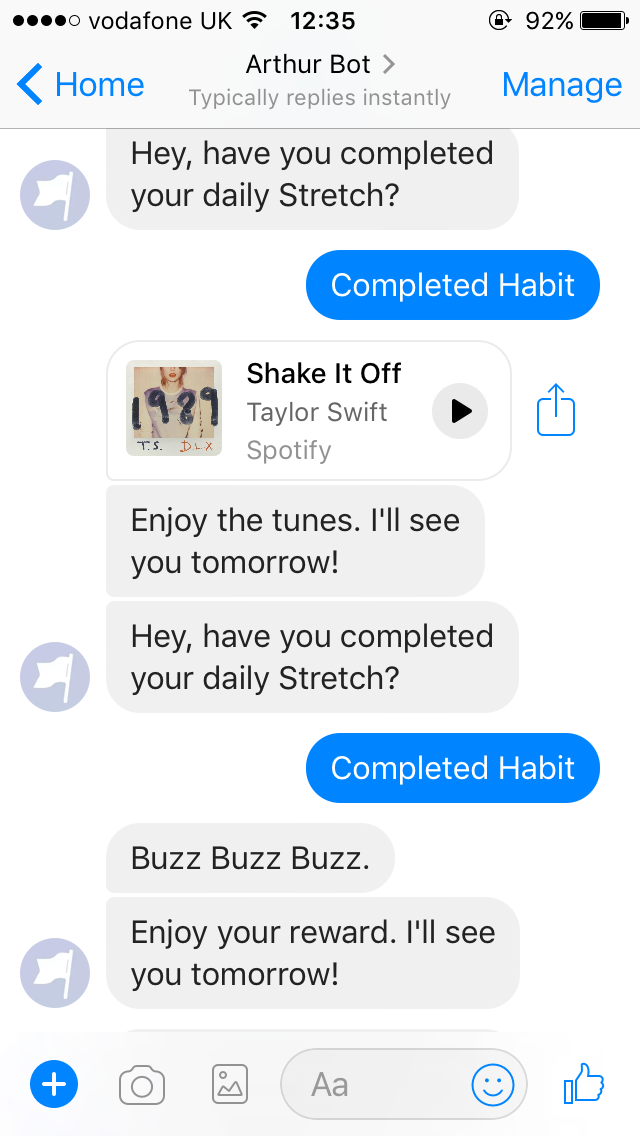
\includegraphics[width=1.8in]{../resources/design/vibration-reward.png}
    \caption{Using vibration as another modality was tested, but due to technical limitations was difficult to implement.}
    \label{fig:vibration_reward_issue}
\end{figure}

Using vibration as a modality would've been a great additional modality to use.
Unfortunately the chatbot sandbox meant that the vibration ability in the phone could not be used, so another device would be used in combination with the bot.
Smart watches and fitness trackers were researched to test if they could programatically vibrate, with the pattern of vibration matching the frequency of the audio.
However, the majority of these devices did not have an API that exposed the vibration element. The best method was found to programatically set an alarm 1-minute into the future using a Fitbit fitness tracker.
This would trigger the vibration when the alarm sounded.
Although this would mean a 1-minute delay after completing a habit, a good user flow could've reduced the wait time with some additional dialogue.
But, this approach relied on the fitness tracker to sync with the phone after the alarm was programatically set. Unfortunately forcing the tracker to sync wasn't available, so this modality was abandoned. Another issue occurred with stopping the audio after it had been played during a reward. If a user closed the reward box, there was no way to stop the audio, unless a user waited until it had finished. This limitation was very minor, but also showed how difficult it is to seemly connect a website and a chatbot. Finally, edge cases throughout interaction were revealed during development and were coded for, for example deciding what would happen if users snoozed their backup notification when it reached the end of the day led to additional logic to stop users from snoozing when it reached the end of the day.


TODO: Go to github issues and paste them into here!

\subsection{Testing}
A test harness was written to perform functional testing on the chatbot. An on-line continuous integration (CI) service was used to programatically run these tests when a \textit{commit} in \textit{version control} was performed on the \textit{master branch}. \textit{Travis CI} (\url{https://travis-ci.org/harrymt/harryshabits}) was used to conduct the tests to ensure the functionality worked throughout development. A pilot trial with five users also tested the basic chatbot functionality preparing for the full evaluation study (Section~\ref{study_comparing_rewards}). Next we evaluate the effectiveness of the prototype against hypotheses in a 4-week study.

\newpage